% template by Natalia Chernov for the University of Oldenburg

\documentclass[xcolor=table,9pt,aspectratio=169]{beamer}

\usepackage[utf8]{inputenc}

\usepackage{anyfontsize}
\usepackage[english,ngerman]{babel}
\usepackage{datetime}
\usepackage{helvet}
   \renewcommand{\familydefault}{\sfdefault}
\usepackage{lipsum}
\usepackage{lmodern}
\usepackage{multicol}
\usepackage{smartdiagram}
\usepackage{tikz}

\definecolor{uolblue}{RGB}{0,62,107}

\definecolor{blue1}{RGB}{0,78,159}
\definecolor{blue2}{RGB}{0,171,217}
\definecolor{blue3}{RGB}{91,197,242}
\definecolor{blue4}{RGB}{161,217,248}

\definecolor{green1}{RGB}{0,120,120}
\definecolor{green2}{RGB}{0,168,121}
\definecolor{green3}{RGB}{148,193,28}
\definecolor{green4}{RGB}{199,211,0}

\definecolor{orange1}{RGB}{213,59,10}
\definecolor{orange2}{RGB}{238,113,0}
\definecolor{orange3}{RGB}{243,145,0}
\definecolor{orange4}{RGB}{253,195,0}

\definecolor{gr}{RGB}{191,191,191}

\setbeamertemplate{frametitle}{\color{uolblue}\fontsize{12}{20}\selectfont{\insertframetitle}}

\pgfdeclareimage[width=0.145\paperwidth]{logo}{figures/slides_logo_uol_negative}
\pgfdeclareimage[width=0.072\paperwidth]{logo_small}{figures/slides_logo_uol_negative}

\defbeamertemplate*{background canvas}{default_page}
{%
\begin{tikzpicture}
   \useasboundingbox (0,0) rectangle (\the\paperwidth,\the\paperheight);
   \filldraw[fill=uolblue,fill opacity=1,draw=none] (0,0) rectangle (0.119\paperwidth,\the\paperheight);
   \filldraw[fill=blue2,fill opacity=1,draw=none] (0.119\paperwidth,0) -- (0.119\paperwidth,0.565\paperheight) arc (117.2:180:0.6\paperwidth) -- cycle;
   \pgftext[at=\pgfpoint{10}{\the\paperheight-11.5},left,top]{\pgfsetfillopacity{1}\pgfuseimage{logo_small}};
\end{tikzpicture}
}
\defbeamertemplate*{background canvas}{titlepage_image}
{
\begin{tikzpicture}
   \useasboundingbox (0,0) rectangle (\the\paperwidth,\the\paperheight);
   \filldraw[fill=uolblue,fill opacity=1,draw=none] (0,0) rectangle (\the\paperwidth,\the\paperheight);
   \filldraw[fill=blue2,fill opacity=1,draw=none] (\the\paperwidth,0) -- (\the\paperwidth,0.66\paperheight) arc (90:180:0.6\paperwidth) -- cycle;
   \pgftext[at=\pgfpoint{14}{\the\paperheight-17.5},left,top]{\pgfsetfillopacity{1}\pgfuseimage{logo}};
\end{tikzpicture}
}
\BeforeBeginEnvironment{frame}{%
   \setbeamertemplate{background canvas}[default_page]%
}
\makeatletter
\define@key{beamerframe}{titlepage_image}[true]{%
   \setbeamercovered{invisible}%
   \setbeamertemplate{background canvas}[titlepage_image]%
}
\makeatother%

\setbeamertemplate{footline}
{
   \leavevmode
   \hbox{
   \hspace*{.025\paperwidth}\begin{beamercolorbox}[wd=.094\paperwidth,ht=2.25ex,dp=1ex,left]{}
   ~

   \vspace*{.042\paperheight}
      \fontsize{4.4}{5.9}\selectfont\color{white}\textbf{Folie \insertframenumber}\newline\insertdate
   \vspace*{.026\paperheight}
   \end{beamercolorbox}
   \hspace*{.05\paperwidth}\begin{beamercolorbox}
   [wd=.79\paperwidth,ht=2.25ex,dp=1ex,left]{}
   ~

   \vspace*{.042\paperheight}
      \fontsize{4.4}{5.9}\selectfont\color{black}\textbf{Empirische Studien zu Fragen der Bedarfsgerechtigkeit}\newline\color{gray}\insertauthor~--~Fakultät IV, Institut für Philosophie
   \vspace*{.026\paperheight}
   \end{beamercolorbox}
   }
   \vskip0pt
}

\setbeamerfont{title}{size={\fontsize{22}{25}}}
\setbeamerfont{subtitle}{size={\fontsize{12}{14}}}
\setbeamerfont{author}{size={\fontsize{9}{11}}}
\setbeamerfont{date}{size={\fontsize{9}{11}}}
\setbeamercolor{title}{fg=white}
\setbeamercolor{subtitle}{fg=white}
\setbeamercolor{author}{fg=white}
\setbeamercolor{date}{fg=white}
\setbeamercolor{color_Logo-Platzhalter}{fg=white,bg=gray!40}

\defbeamertemplate*{title page}{customized}[1][]
{  \vspace*{20mm}
   \hspace*{-22.5mm}
   \begin{minipage}{\textwidth}
   \usebeamerfont{title}\usebeamercolor[fg]{title}\inserttitle\par
   \bigskip
   \usebeamerfont{subtitle}\usebeamercolor[fg]{subtitle}\insertsubtitle\par
   \bigskip
   \usebeamerfont{author}\usebeamercolor[fg]{author}\insertauthor,
   \usebeamerfont{date}\usebeamercolor[fg]{date}\insertdate\par
   \end{minipage}
}
\setbeamertemplate{navigation symbols}{}
\setbeamersize{text margin left=0.17\paperwidth,text margin right=0.04\paperwidth}

\title{Empirische Studien zu Fragen\\der Bedarfsgerechtigkeit}
\subtitle{}
\author{Alexander Max Bauer}
\date{\renewcommand{\dateseparator}{.}\ddmmyyyydate\today}
\usepackage{enumitem}
\def\labelitemi{--}
\def\labelitemii{--}
\def\labelitemiii{--}

\begin{document}
{
\setbeamertemplate{footline}{}
\begin{frame}[titlepage_image]
   \maketitle
\end{frame}
}


%%%%%%%%%%%
% FOLIE 2 %
%%%%%%%%%%%
\begin{frame}{\vspace*{10mm}Gliederung}
\vspace*{-10mm}
\begin{itemize}
   \item[(1)] Vorgeschichte
   \item[(2)] Empirische Forschung und normative Theorie \textcolor{gray}{(Bauer und Meyerhuber 2019)}
   \item[(3)] Bedarf und Bedarfsgerechtigkeit \textcolor{gray}{(Bauer 2019)}
   \item[(4)] Bedarf als Referenzpunkt \textcolor{gray}{(Bauer et al. 2023a)}
   \item[(5)] Bedarf und Verantwortung \textcolor{gray}{(Bauer et al. 2022)}
   \item[(6)] Bedarfsarten \textcolor{gray}{(Bauer et al. 2023b)}
   \item[(7)] Zusammenfassung zentraler Ergebnisse
\end{itemize}
\end{frame}


%%%%%%%%%%%
% FOLIE 3 %
%%%%%%%%%%%
\begin{frame}{\vspace*{10mm}Vorgeschichte}
\frame{
\includegraphics[width=0.8\linewidth]{figures/slides_email.png}}
\end{frame}


%%%%%%%%%%%
% FOLIE 4 %
%%%%%%%%%%%
\begin{frame}{\vspace*{10mm}Vorgeschichte}
\frame{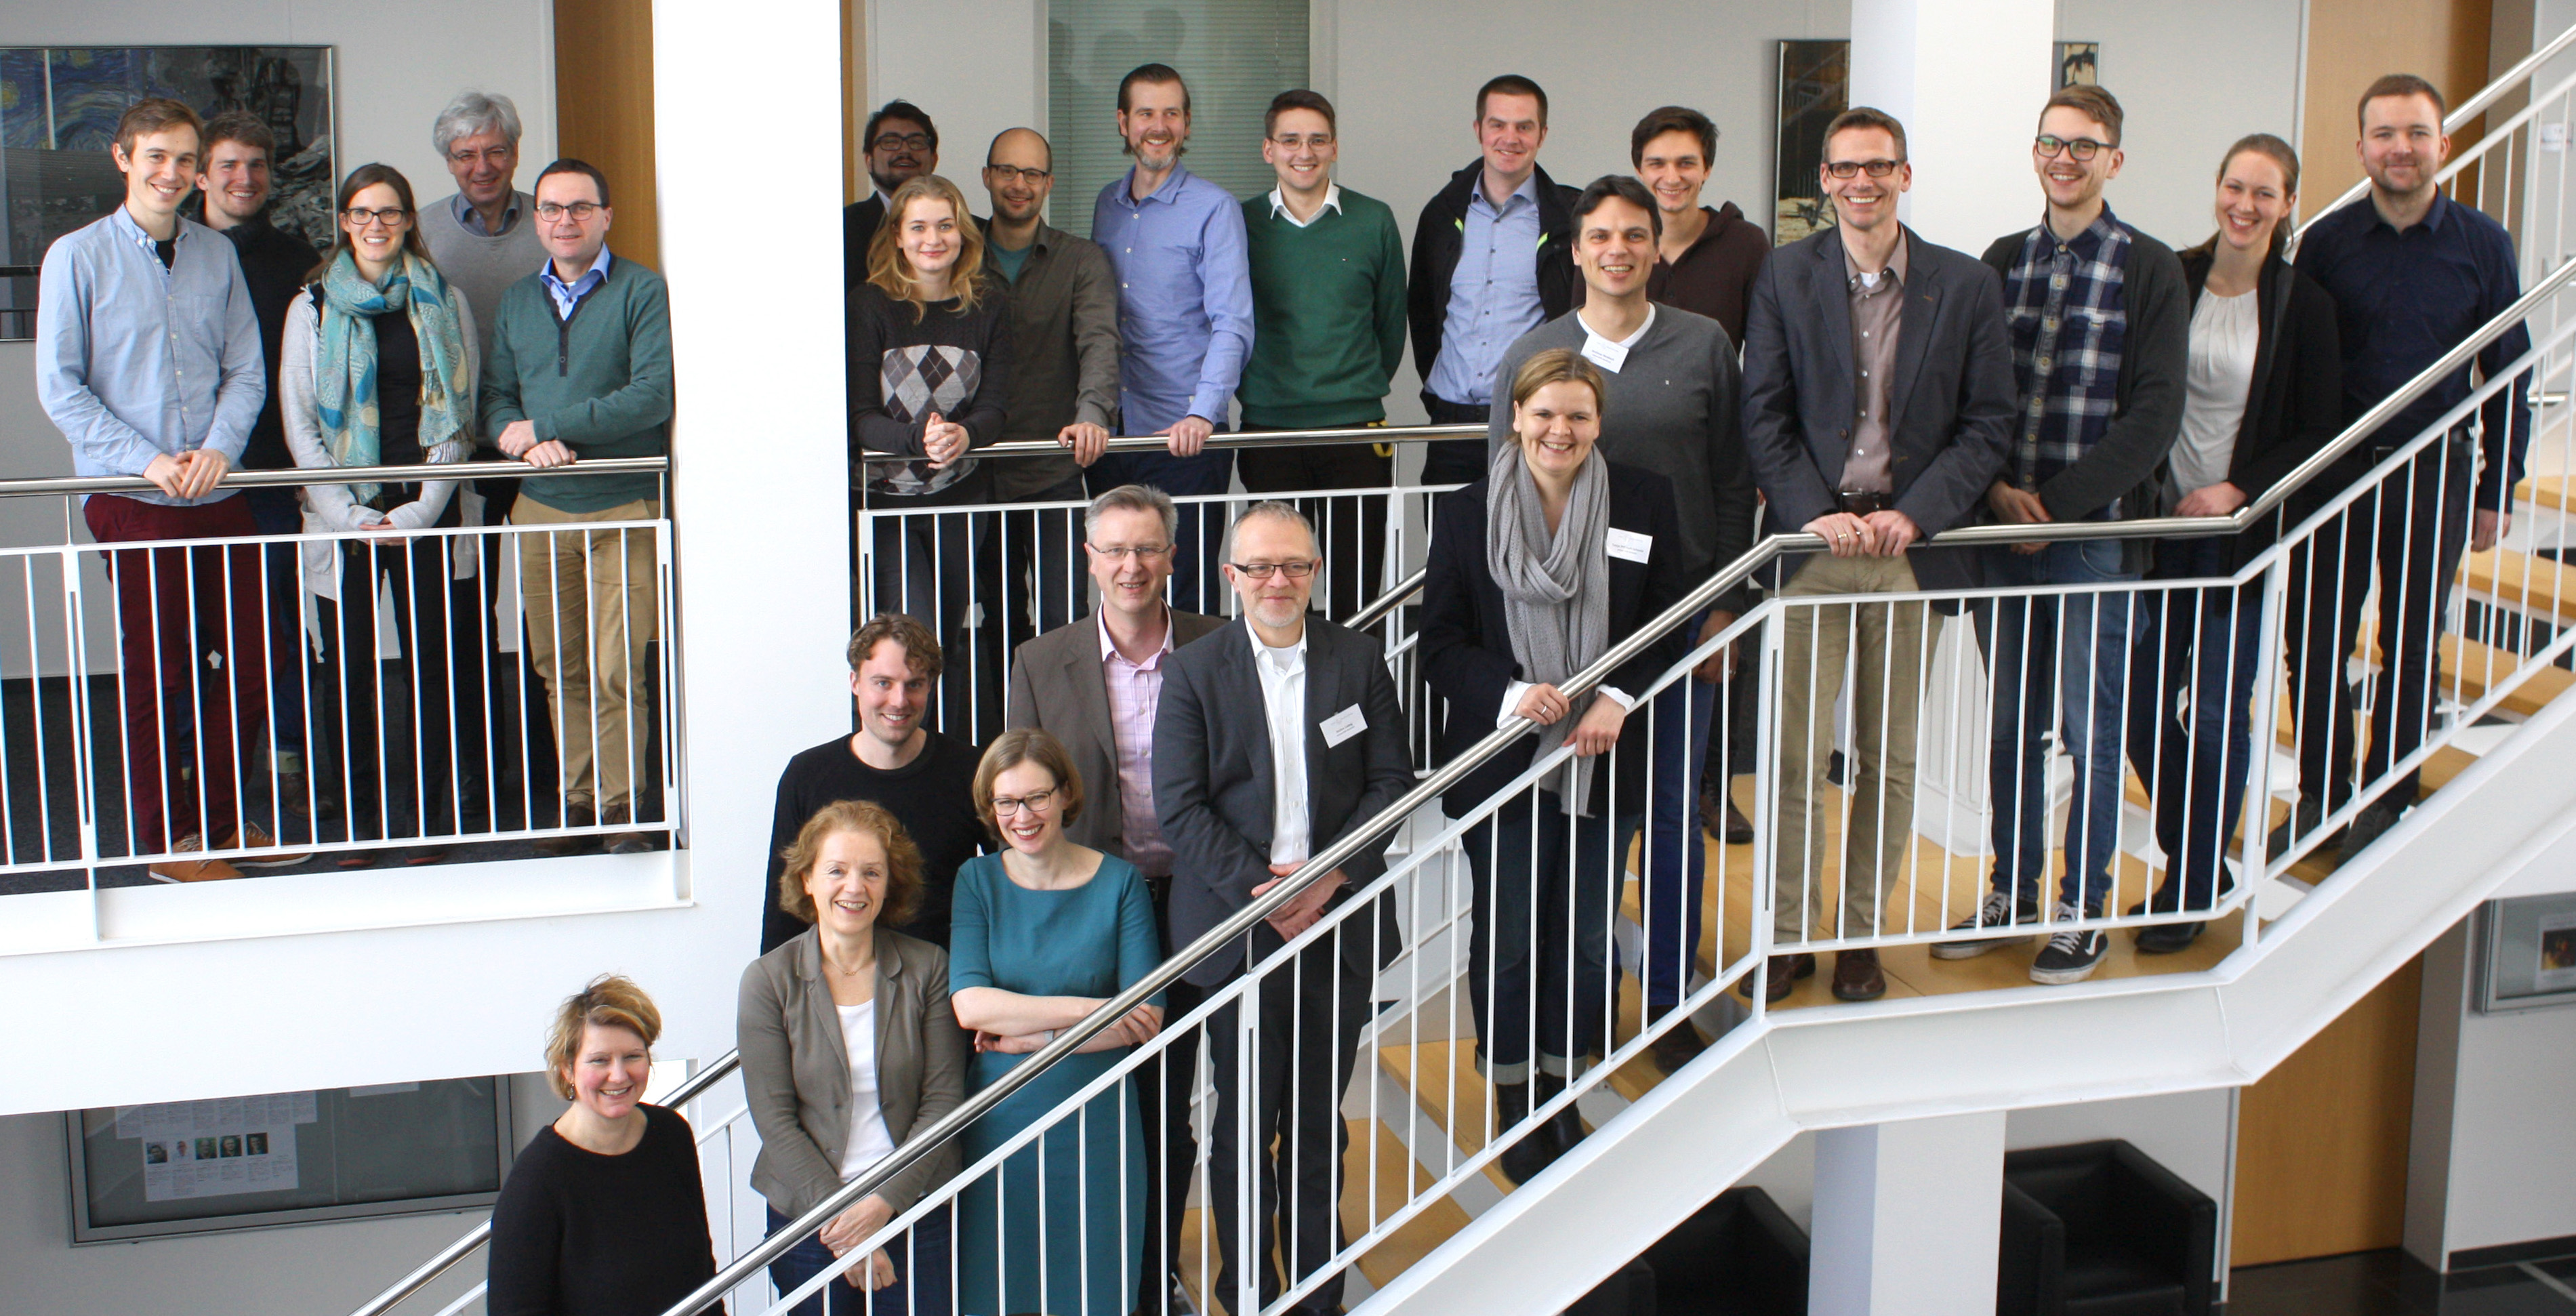
\includegraphics[width=0.8\linewidth]{figures/slides_for.jpg}}
\end{frame}


%%%%%%%%%%%
% FOLIE 5 %
%%%%%%%%%%%
\begin{frame}{\vspace*{10mm}Vorgeschichte}
\frame{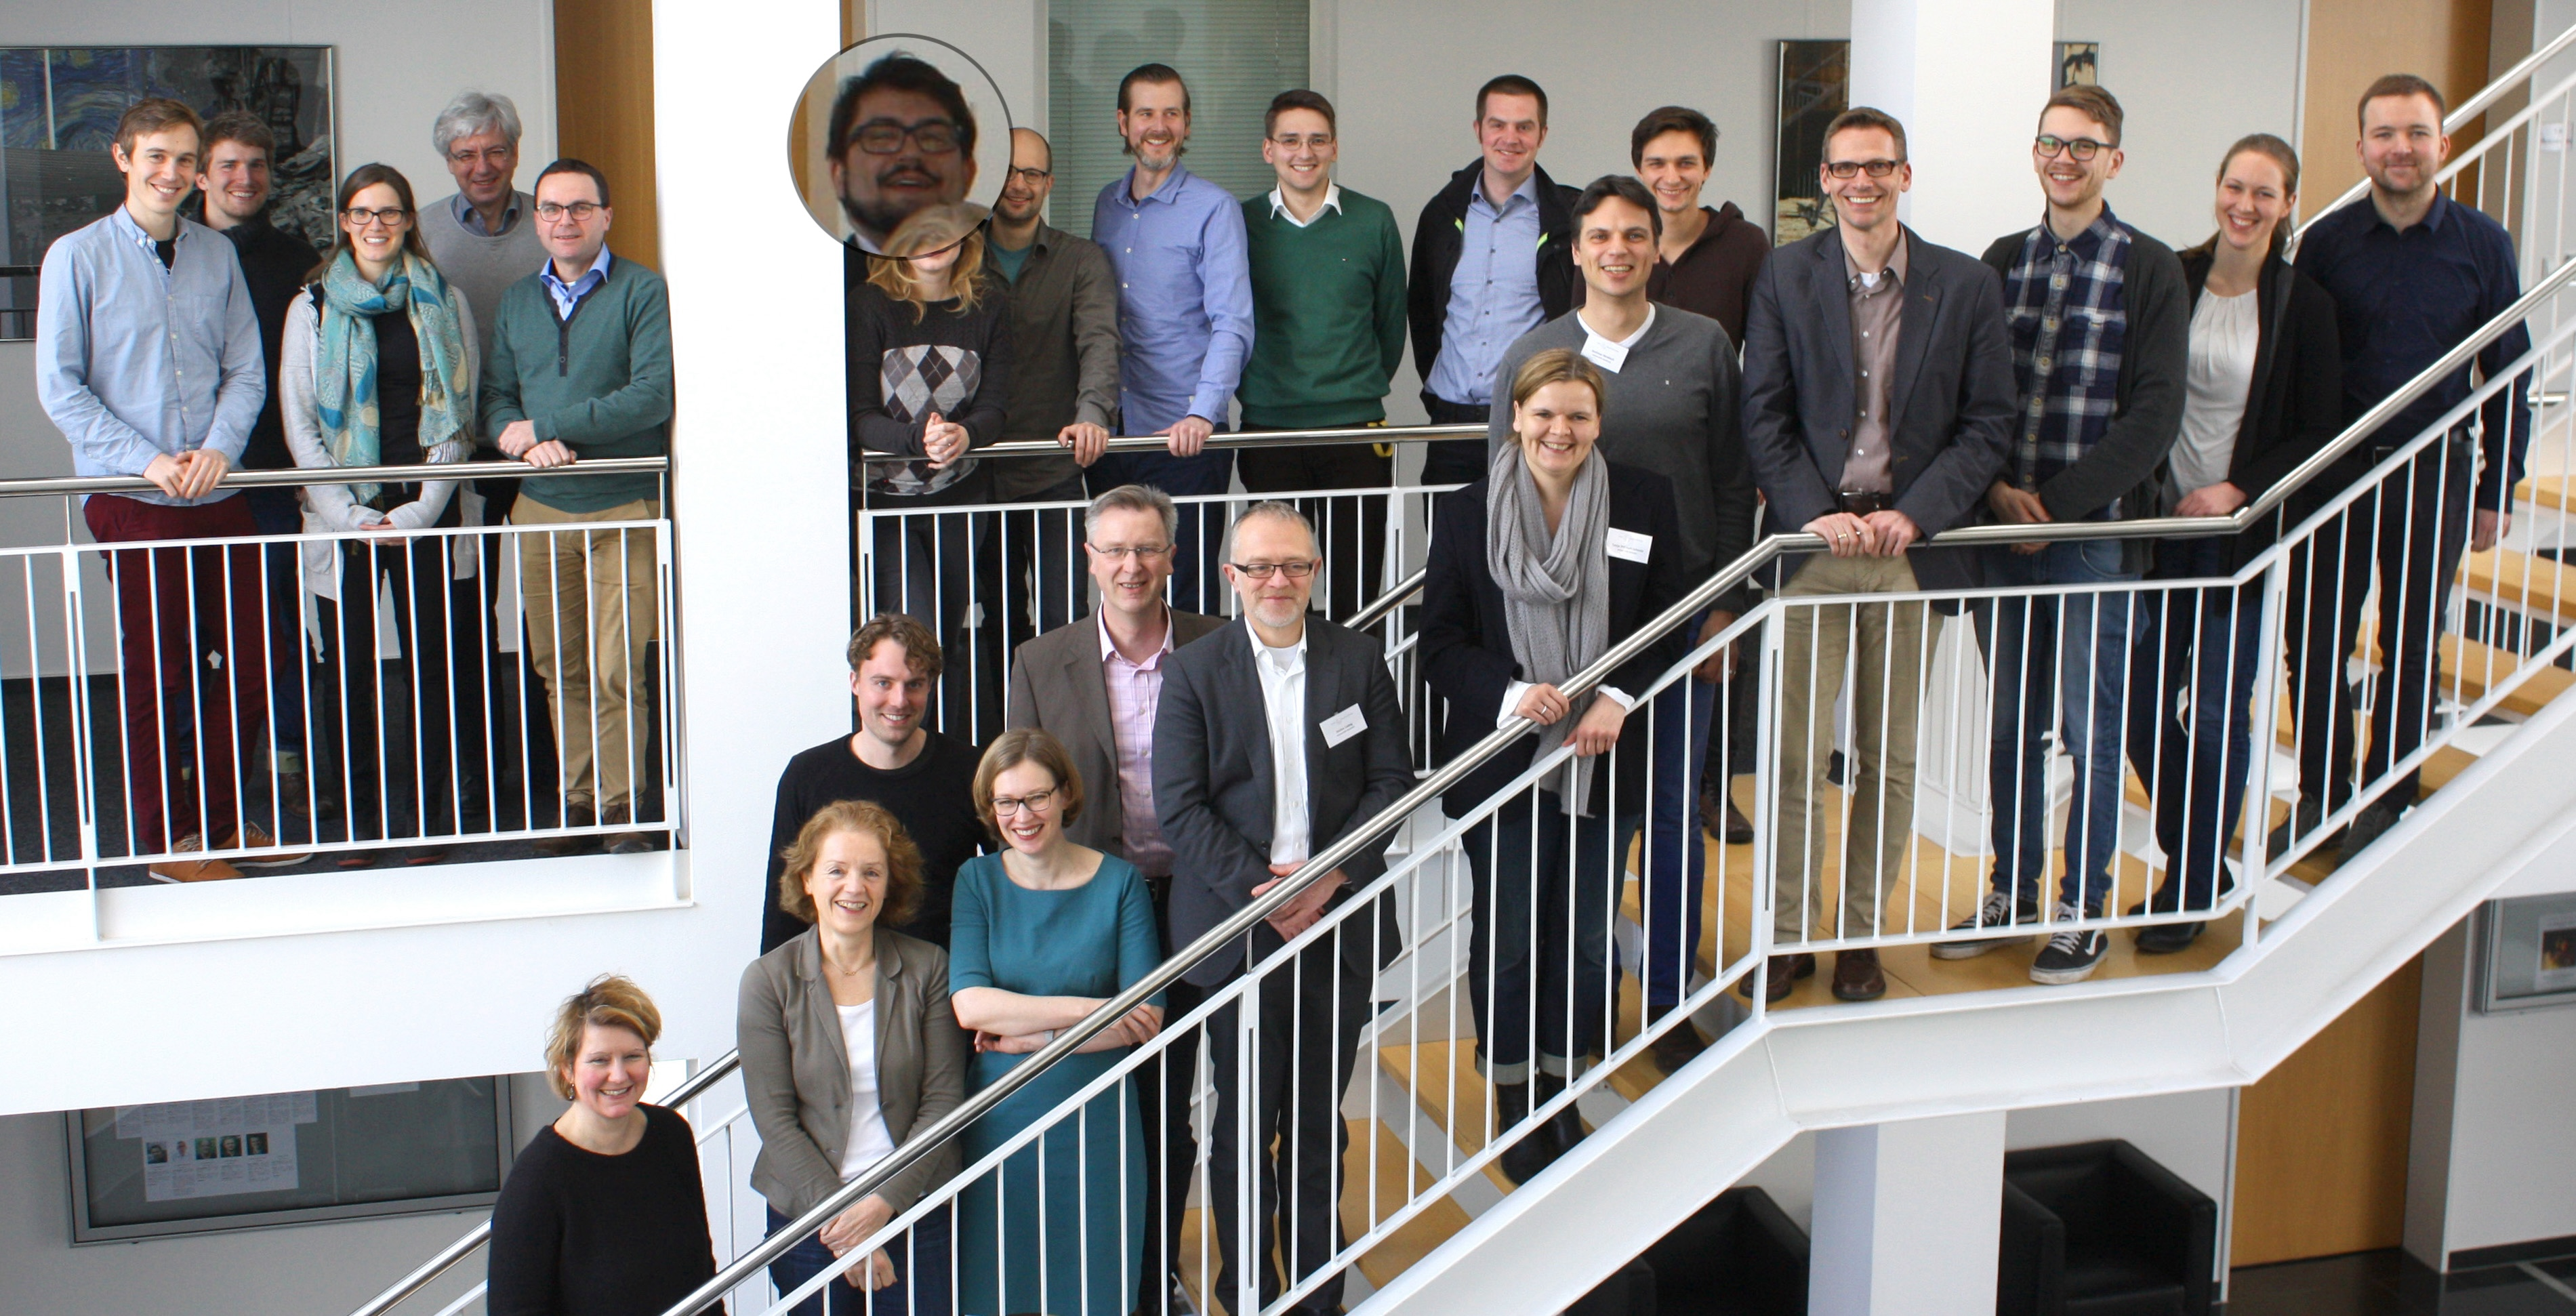
\includegraphics[width=0.8\linewidth]{figures/slides_for_close_up.jpg}}
\end{frame}


%%%%%%%%%%%
% FOLIE 6 %
%%%%%%%%%%%
\begin{frame}{\vspace*{10mm}Empirische Forschung und normative Theorie}
\begin{itemize}
   \item[(E1)] Deskriptive Ethik $\in$ Experimentelle Philosophie
   \item[(E2)] Experimentelle Philosophie $\in$ Philosophie
\end{itemize}
\end{frame}


%%%%%%%%%%%
% FOLIE 7 %
%%%%%%%%%%%
\begin{frame}{\vspace*{10mm}Empirische Forschung und normative Theorie}
\begin{multicols}{2}
\begin{itemize}
   \item[(E3)] Experimentelle Philosophie kann einen Beitrag zur normativen Ethik leisten
   \begin{itemize}
      \item[(E3.1)] Erweiterung der Grundgesamtheit an Introspektionen, die zur Reflexion zur Verfügung stehen
      \item[(E3.2)] Ipsum
   \end{itemize}
\end{itemize}
\vfill

\begin{center}
   \vspace{1cm}
   \frame{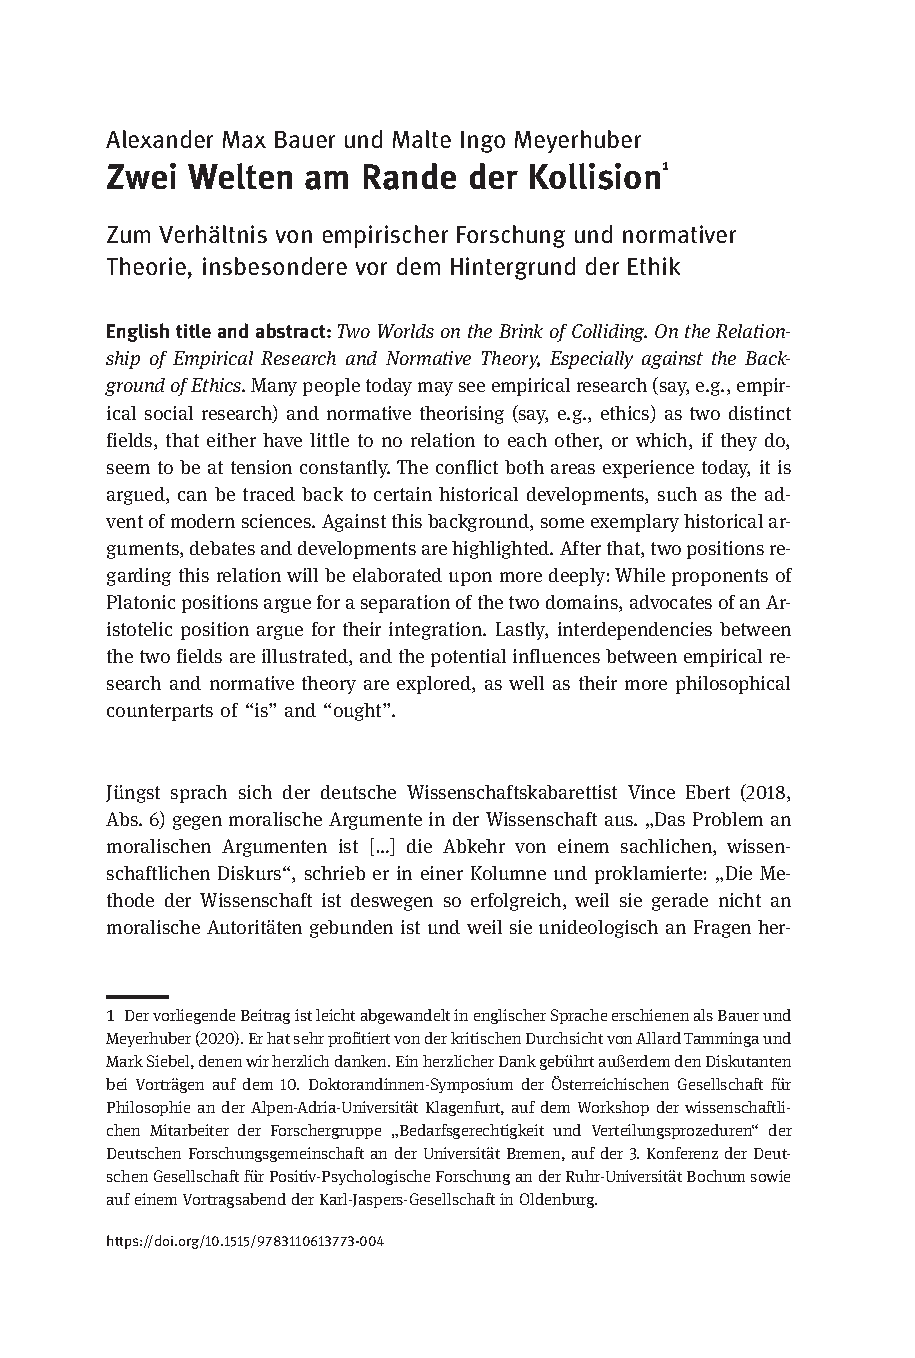
\includegraphics[width=0.6\linewidth]{figures/slides_bauer_meyerhuber_2019.pdf}}
   \vspace{1cm}
\end{center}
\end{multicols}
\end{frame}


%%%%%%%%%%%
% FOLIE 8 %
%%%%%%%%%%%
\begin{frame}{\vspace*{10mm}Bedarf und Bedarfsgerechtigkeit}
\begin{multicols}{2}
\begin{itemize}
   \item Lorem
   \item Ipsum
   \item Dolor
\end{itemize}
\vfill

\begin{center}
   \vspace{1cm}
   \frame{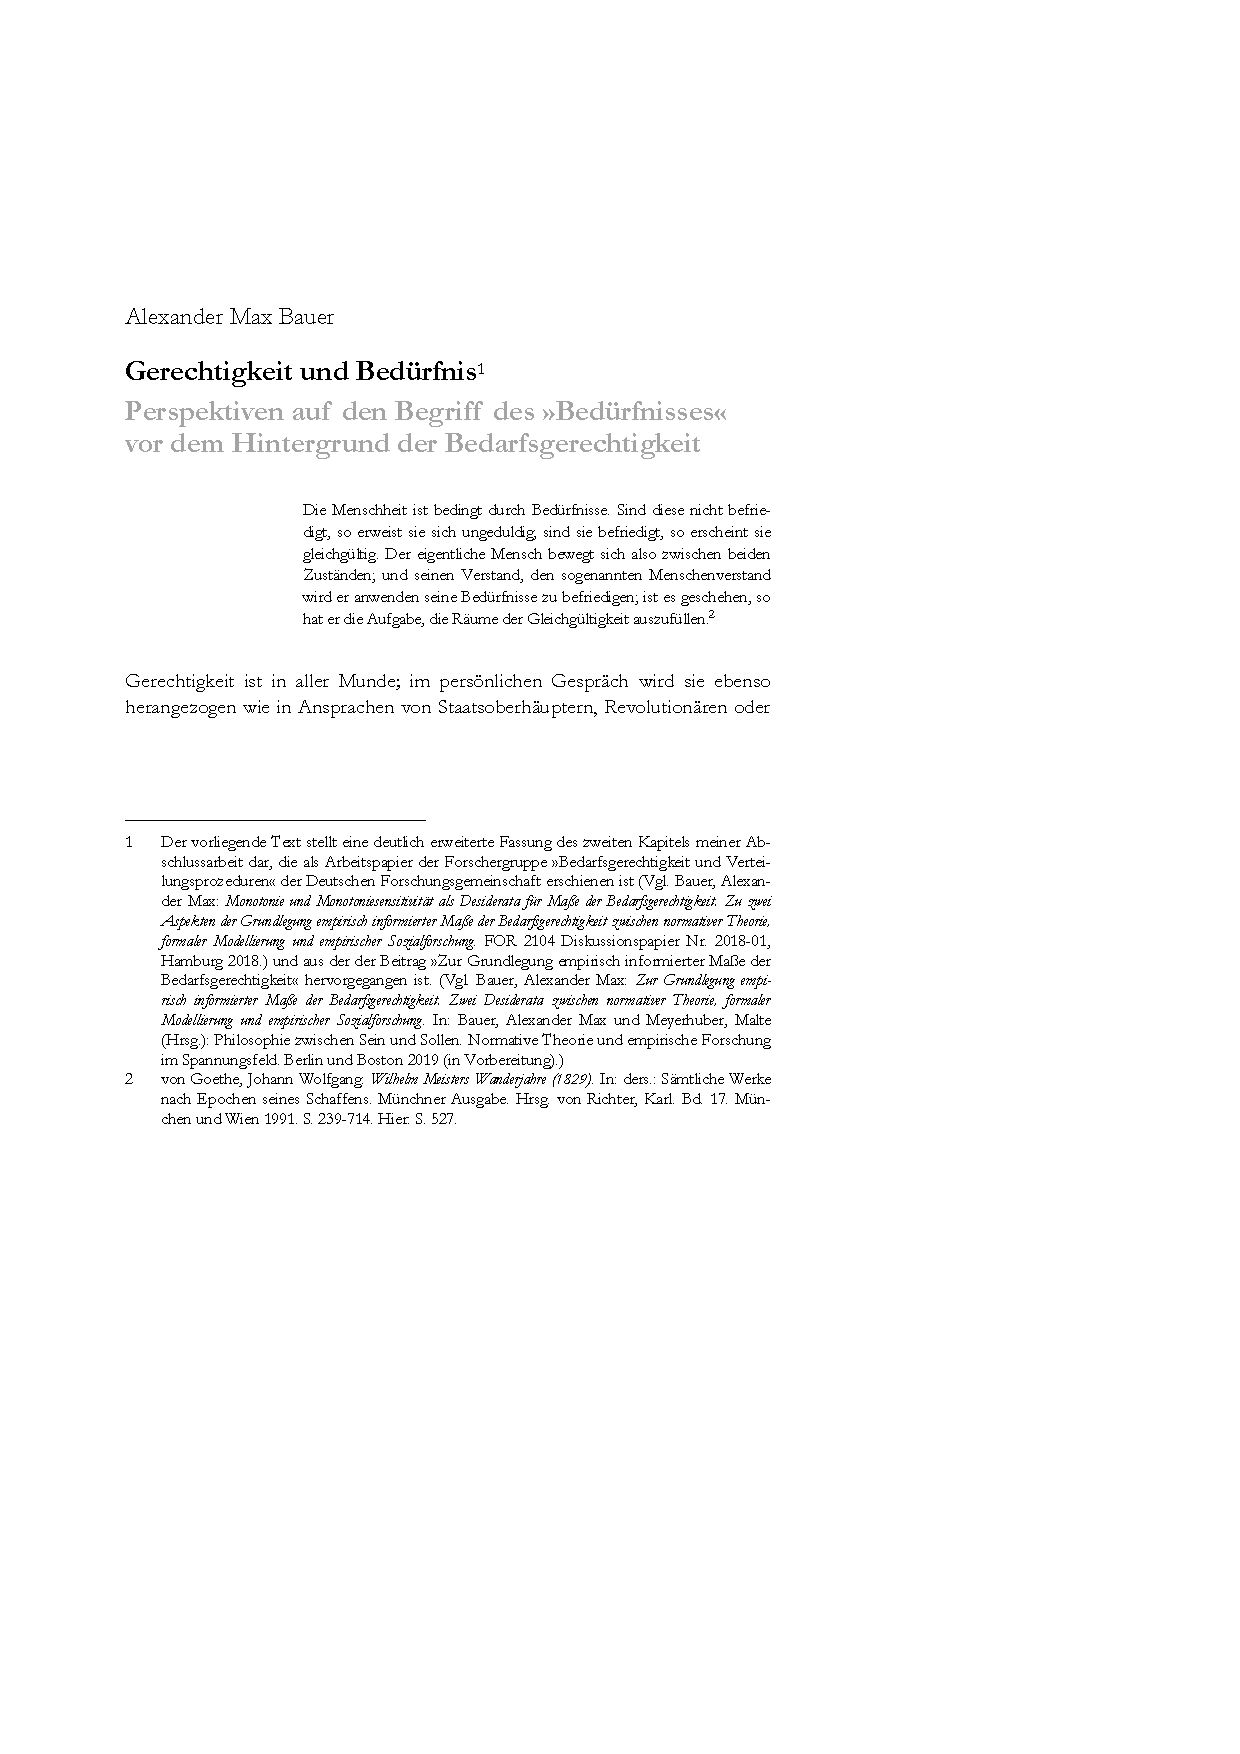
\includegraphics[width=0.6\linewidth]{figures/slides_bauer_2019.pdf}}
   \vspace{1cm}
\end{center}
\end{multicols}
\end{frame}


%%%%%%%%%%%
% FOLIE 9 %
%%%%%%%%%%%
\begin{frame}{\vspace*{10mm}Bedarf als Referenzpunkt}
\begin{multicols}{2}
\begin{itemize}
   \item Lorem
   \item Ipsum
   \item Dolor
\end{itemize}
\vfill

\begin{center}
   \vspace{1cm}
   \frame{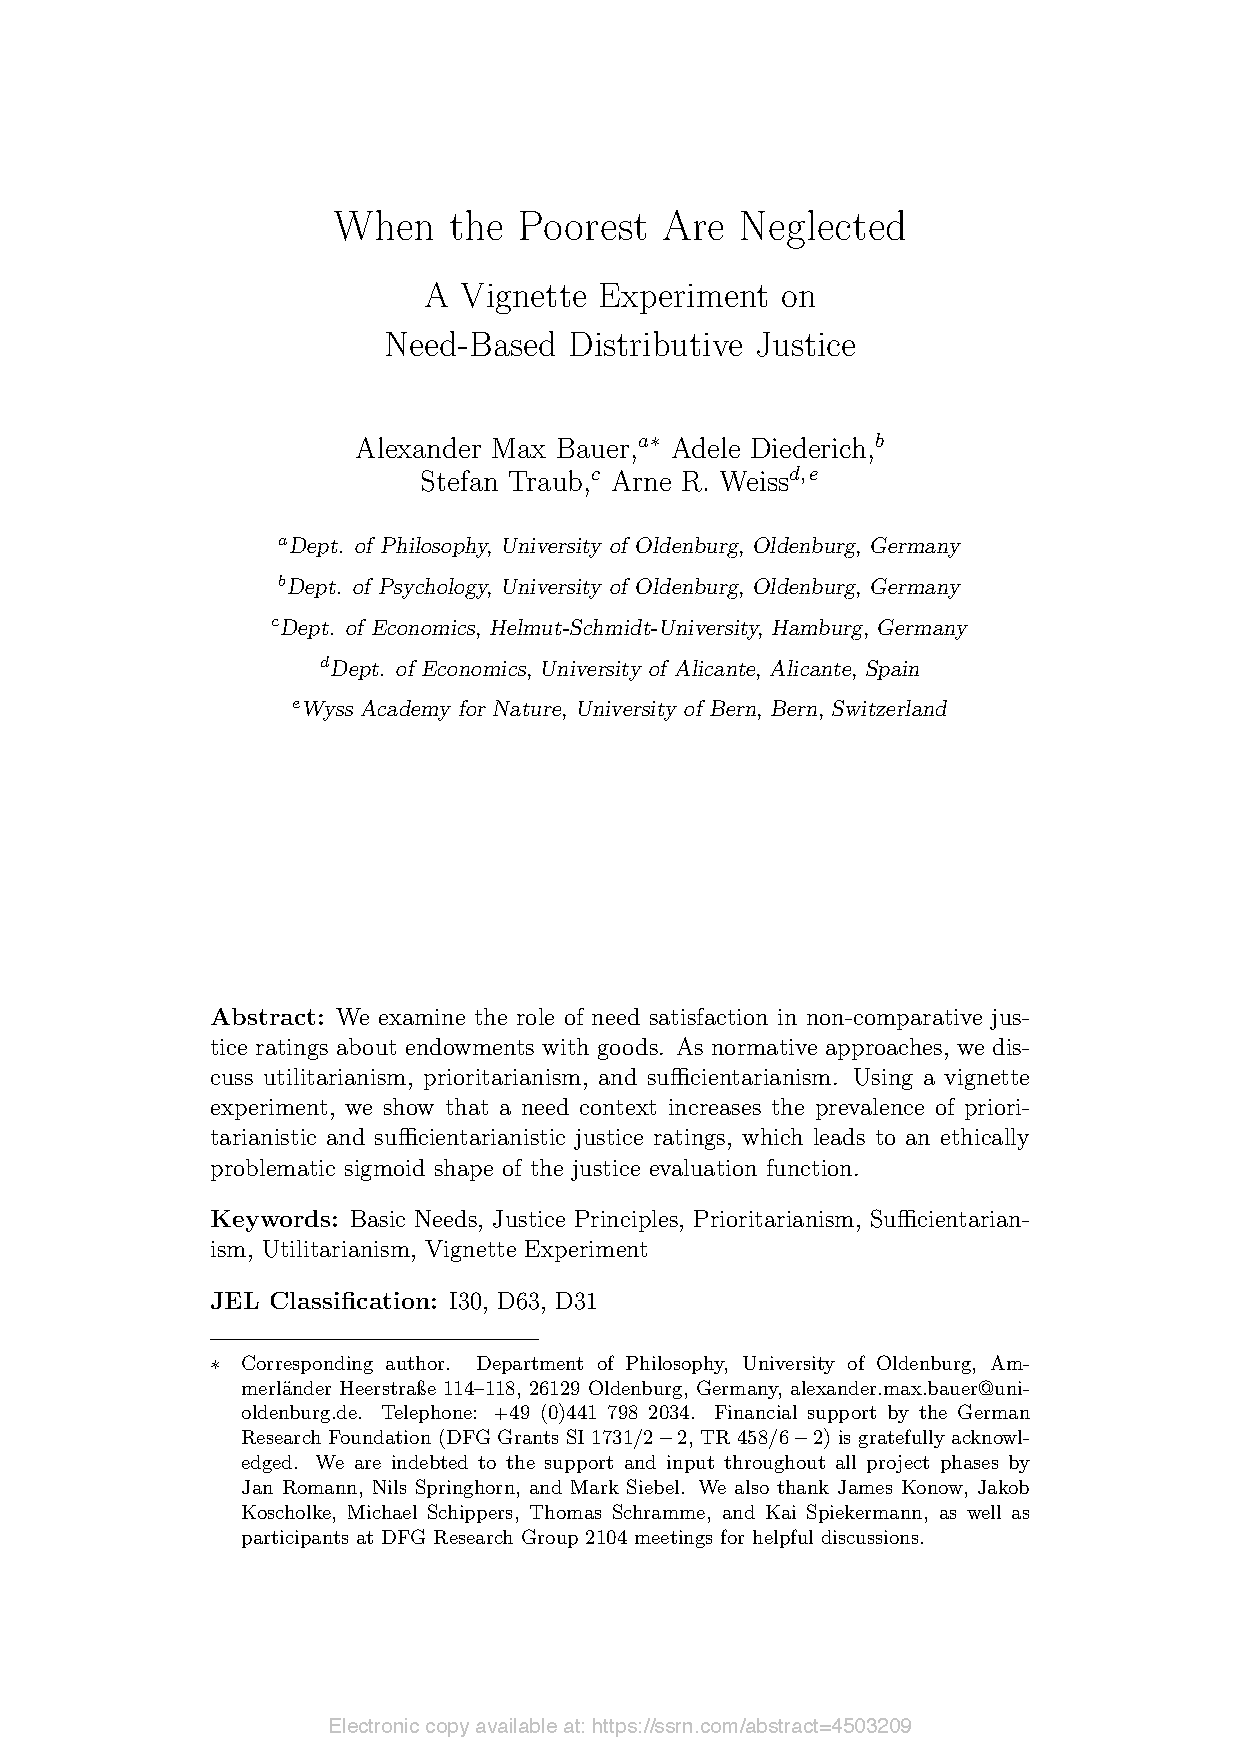
\includegraphics[width=0.6\linewidth]{figures/slides_bauer_et_al_2023a.pdf}}
   \vspace{1cm}
\end{center}
\end{multicols}
\end{frame}


%%%%%%%%%%%%
% FOLIE 10 %
%%%%%%%%%%%%
\begin{frame}{\vspace*{10mm}Bedarf und Verantwortung}
\begin{multicols}{2}
\begin{itemize}
   \item Lorem
   \item Ipsum
   \item Dolor
\end{itemize}
\vfill

\begin{center}
   \vspace{1cm}
   \frame{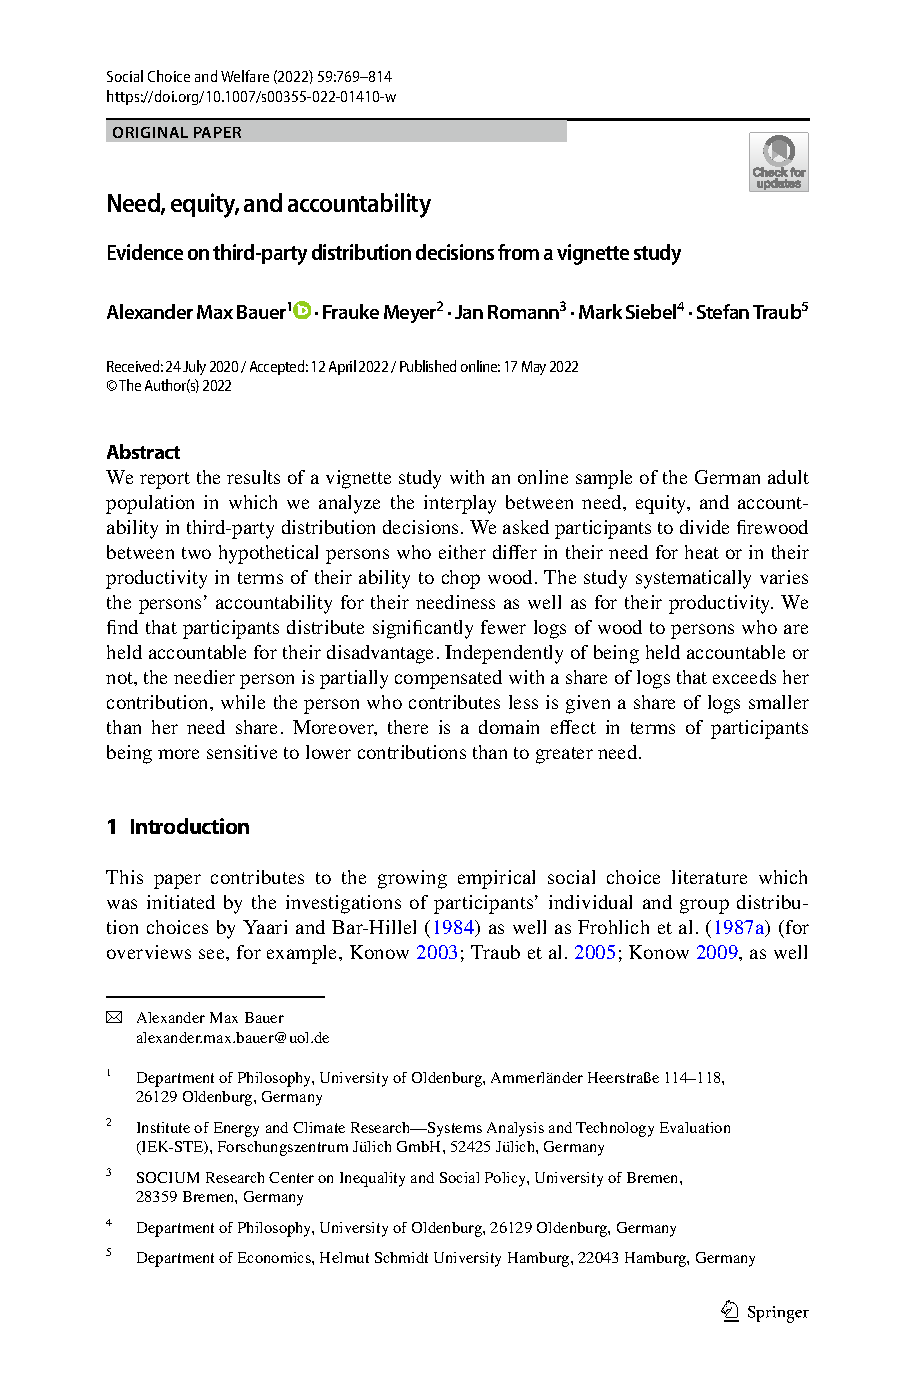
\includegraphics[width=0.6\linewidth]{figures/slides_bauer_et_al_2022.pdf}}
   \vspace{1cm}
\end{center}
\end{multicols}
\end{frame}


%%%%%%%%%%%%
% FOLIE 11 %
%%%%%%%%%%%%
\begin{frame}{\vspace*{10mm}Bedarfsarten}
\begin{multicols}{2}
\begin{itemize}
   \item Lorem
   \item Ipsum
   \item Dolor
\end{itemize}
\vfill

\begin{center}
   \vspace{1cm}
   \frame{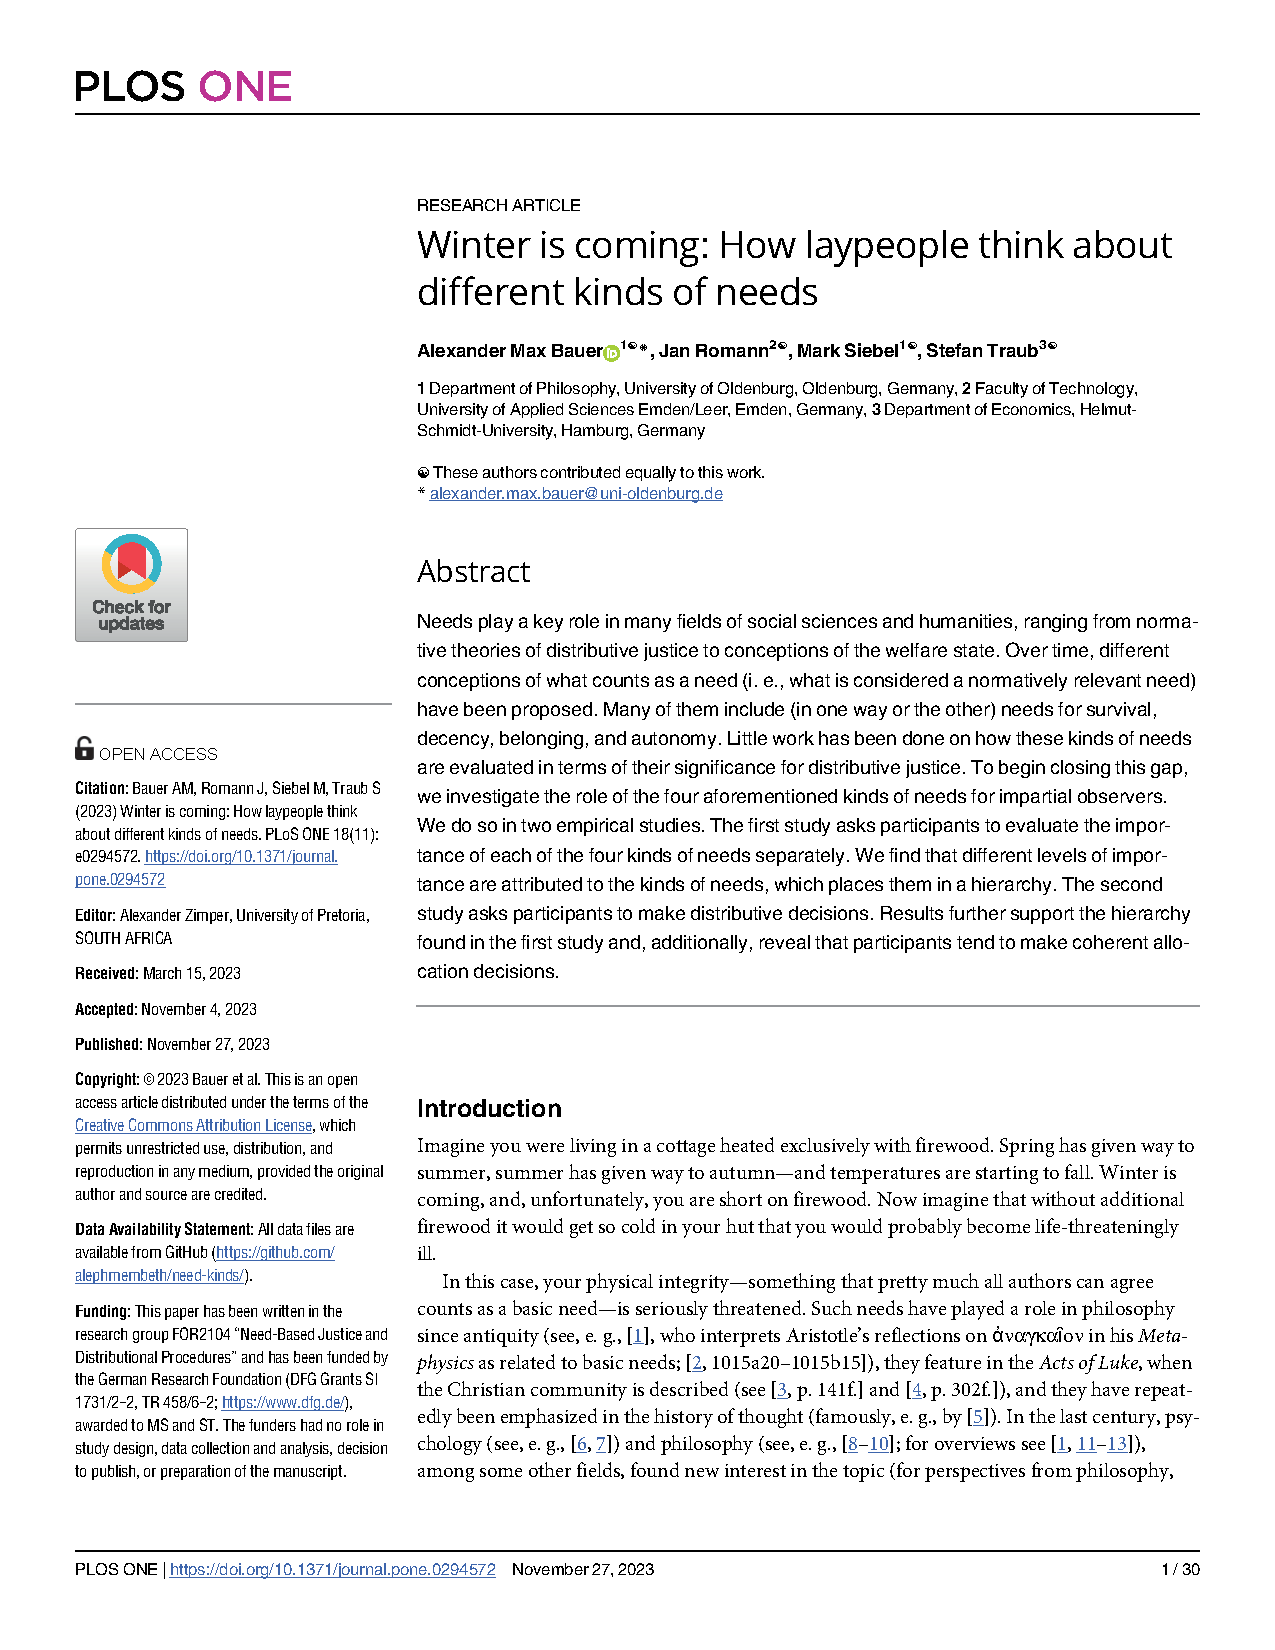
\includegraphics[width=0.6\linewidth]{figures/slides_bauer_et_al_2023b.pdf}}
   \vspace{1cm}
\end{center}
\end{multicols}
\end{frame}


%%%%%%%%%%%%
% FOLIE 12 %
%%%%%%%%%%%%
\begin{frame}{\vspace*{10mm}Zusammenfassung zentraler Ergebnisse}
\vspace*{-10mm}
\begin{itemize}
   \item[(1)] Unparteiische Beobachter*innen nehmen graduelle Gerechtigkeitseinschätzungen vor
   \item[(2)] Diese Einschätzungen sind abhängig von Versorgungssituationen
   \item[(3)] Bedarfsinformationen beeinflussen diese Einschätzungen
\end{itemize}

\vspace{1em}
\begin{itemize}
   \item[(4)] Unparteiische Entscheider*innen berücksichtigen Bedarf, Leistung und Verantwortung
   \item[(5)] Auch bei zu geringer Leistung wird Bedarf teilweise kompensiert
   \item[(6)] Kompensationsbereitschaft sinkt, wenn zu geringe Leistung selbst verschuldet ist
\end{itemize}

\vspace{1em}
\begin{itemize}
   \item[(7)] Unparteiische Beobachter*innen und Entscheider*innen unterscheiden Bedarfsarten
\end{itemize}
\end{frame}

\end{document}
